%!TEX root = PMP_ClockPendulumAnalyzer.tex
\section{Test}
		\subsection{Testumgebung}
        Der Pendulum Analyzer wird mittels einer normalen Wand-Pendeluhr getestet. Dazu wird die Uhr in einer dafür hergestellten Verschalung aufgehängt.
        \begin{figure}[H]
            \centering
            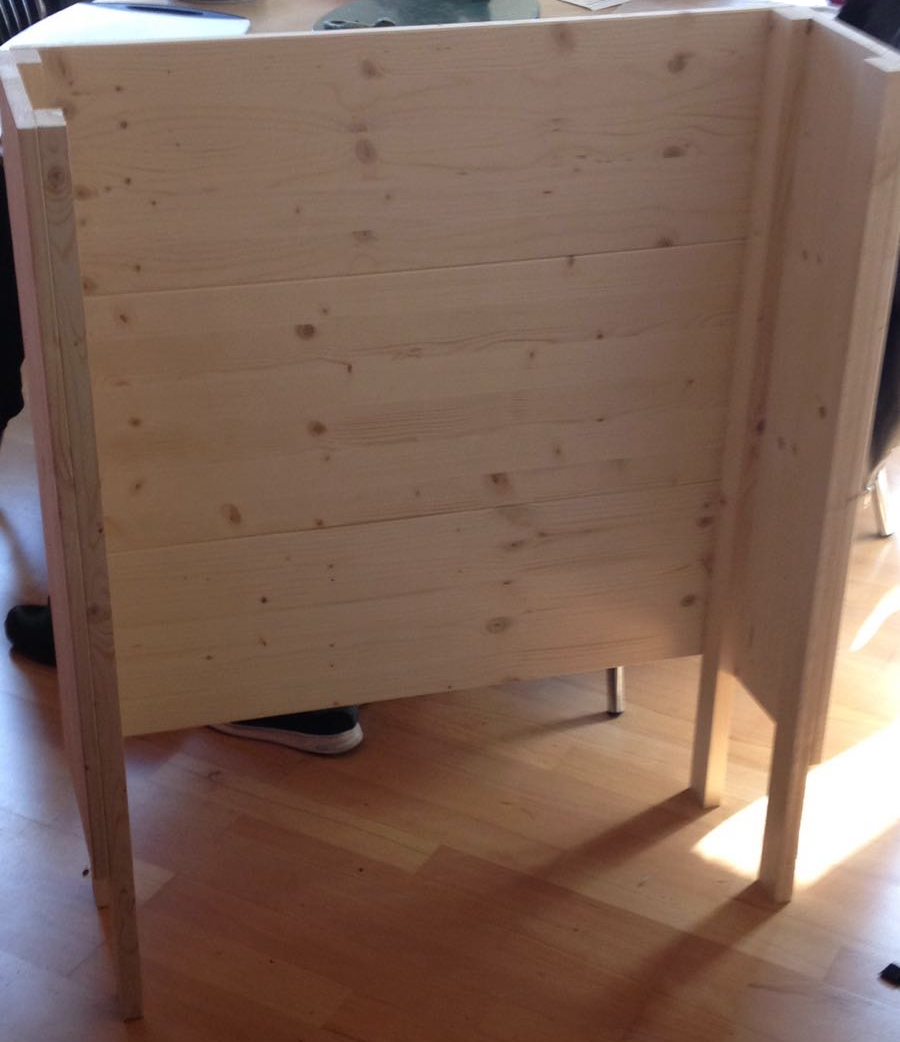
\includegraphics[width=.5\textwidth]{verschalung.png}
            \caption{Verschalung für die Pendeluhr}
        \end{figure}

        \noindent Die Uhr hat eine Fläche auf der das Gerät platziert werden kann. Es wird daher keine zusätzliche Montage für die Sensoren gebaut.
		\subsection{Testfälle}
			\textit{Was wird durch das Testen abgedeckt}
			\subsubsection{Unit Tests}
			\subsubsection{Blackbox Tests}